
\chapter{Einleitung}

Dieses Kapitel soll den Leser auf den Inhalt der Arbeit aufmerksam machen, ihn mit der Aufgabestellung vertraut machen und "uber die Strukturierung und Zielsetzung der Arbeit Auskunft geben.


\section{Motivation}
Objekte werden in der heutigen Tagen immer mehr mit Elektronik und Intelligenz versehen. Die Leute wollen aufgrund dieser Entwicklung, dass Prozesse oder bestimmte Aufgaben ohne menschliches Eingreifen erledigt und miteinander vernetzt werden. Das System soll nur "uberwacht werden und die Ergebnisse zu bestimmten Zwecken benutzt werden.

Das Internet der Dinge (in Englisch \textbf{\textit{internet of things}}, Kurzform \textbf{IoT}) wird dazu benutzt, um die Interaktion zwischen Menschen und vernetzten elektronischen Systemen zu vereinfachen. 


\section{Aufgabenstellung und Zielsetzung}
Diese Bachelorarbeit besch"aftigt sich mit der Entwicklung eines vernetzten Systems bestehend aus einem 3D-Beschleunigungssensor, einem 3D-Gyroskop sowie einem Tem\-peratur- und Feuchtigkeitssensor. Die Sensoren messen Daten und "ubergeben diese an den STM32L475 Mikrocontroller.

Der Mikrocontroller soll die Daten verarbeiten und mit Hilfe von einem LoRa-Modul\cite{AT_Command} drahtlos zu einem Server "ubertragen. Bevor die "Ubertragung erfolgt, muss das LoRa-Modul Zugang zu dem Server durch ein Gateway bekommen. Abbildung \ref{LRWAN} gibt einen "Uberblick "uber den Aufbau des gesamten Systems.

% Bild hinzufügen 
\begin{figure}[h]	
	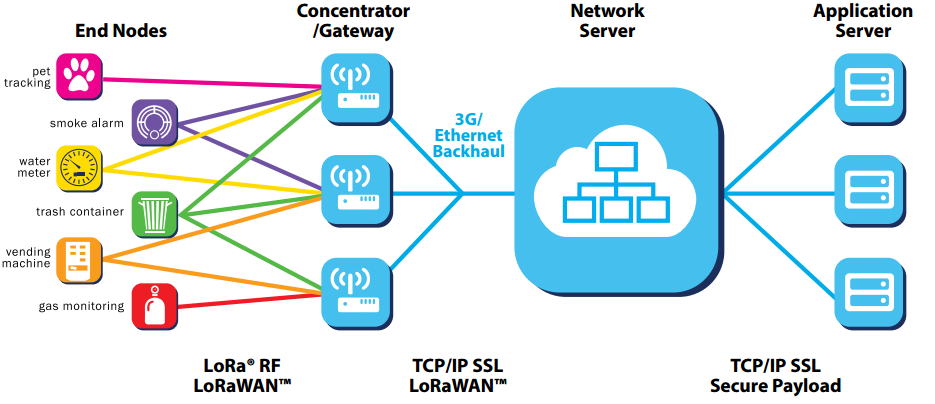
\includegraphics[width=15cm]{source/images/LoRaWAN_NET}
	\caption{LoRaWAN Netzwerkarchitektur \cite{LoRaWAN}}\label{LRWAN}
\end{figure}

\vspace{5cm}

\section{Gliederung der Arbeit}

Das Kapitel \ref{Komponente} gibt einen detaillierten "Uberblick "uber allen Hardware-Komponenten, die bei der Durchf"uhrung dieser Arbeit verwendet werden. Hinzu kommt die Erl"auterung der Software-Entwicklung. Als Erstes wird auf die Eigenschaften von des benutzten STM32-Nucleo Board eingegangen. Diesem Kapitel ist auch zu entnehmen, warum genau dieses Board gew"ahlt wurde. 

Als n"achstes wird das LoRa Node und das LoRaWAN-Protokoll beschrieben. Dieser LoRa-Node wird dazu verwendet, um die gesammelten Daten dem Server drahtlos zu "ubertragen.

Das Kapitel \ref{G_S} beschreibt wie der LoRaWAN-Server und das Gateway funktionieren und zeigt die Konfigurationen, die zu "ubernehmen sind, um eine Verbindung mit einem LoRa-Node herzustellen.

Anschlie\ss{}end im Kapitel \ref{Fazit} wird eine Zusammenfassung und einen kleinen Ausblick der Arbeit gegeben.
   